\documentclass[10pt]{article}
\usepackage{preamble}

\def\FS{Formelsammlung}
\def\Fach{Felder, Wellen und Leitungen}
\title{\FS \ \Fach}
\date{\today}
\def\Semester{Sommersemester 22}
\IfFileExists{info.tex}
{
    \input{info.tex}
}
{
    \author{\href{https://www.youtube.com/watch?v=yMR45cZbvDw}{Die Prinzen - Alles nur geklaut}}
    \def\MatNr{MATNR}
}

\begin{document}

\pagenumbering{gobble}
\begin{titlepage}
    \thispagestyle{empty}

    \begin{center}
        
\includegraphics[width=0.7\textwidth]{OTHR_OTHR_Logo}\\
        \vspace*{\stretch{1}}
        \Huge
        \textsc{\MyTitle}\\
        \vspace*{\stretch{0.25}}
        \normalsize
        \Semester

        \vspace*{\stretch{2}}
        {\renewcommand{\arraystretch}{1.5}
            \begin{tabular}{l l}
                Name:            & \hspace{4cm}\MyAuthor \\
                Matrikelnummer:  & \hspace{4cm}\MatNr    \\
                Letzte Änderung: & \hspace{4cm}\MyDate   \\
                Lizenz:          & \hspace{4cm}GPLv3
            \end{tabular}
        }
        \vspace*{\stretch{1}}

    \end{center}
\end{titlepage}

\newpage


\tableofcontents\clearpage

\pagestyle{fancy}
\lhead{\MyAuthor}
\rhead{\Semester}
\cfoot{\vspace{-20pt}\thepage}
\pagenumbering{arabic}
% \setlength{\columnsep}{1pt}
\raggedcolumns


\begin{multicols*}{2}
    \section{Grundlagen}

\subsection{Randbedingung}
\begin{tabularx}{0.45\textwidth}{>{\hsize=.3\hsize}X|>{\hsize=.7\hsize}X}
    Dirichlet-RB & Funktion nimmt an den Rändern einen bestimmten Wert an (Bsp.: $\rho_r = 5V$)\\
    \hline
    Neumann-RB &  Die Normalableitung der Fkt. nimmt an den Rändern einen bestimmten Wert an\\
\end{tabularx}

\subsection{Begriffe}
\begin{tabularx}{0.45\textwidth}{>{\hsize=.2\hsize}X|>{\hsize=.4\hsize}X|>{\hsize=.4\hsize}X}
        & Begriff & Beschreibung \\
    \hline
    $\rho$ &  &  \\
\end{tabularx}

\subsection{Kartesische Koordinaten}
Einheitsvektoren:   $\quad \vec{e_{x}}, \vec{e_{y}}, \vec{e_{z}}$\\ 
Rechtssystem:       $\vec{e_{x}} \times \vec{e_{y}}=\vec{e_{z}}$\\
Linienelemente:     $\quad d s=\sqrt{d x^{2}+d y^{2}+d z^{2}}$\\
Nabla Operator:     $\quad \nabla=\frac{\partial}{\partial x} \vec{e_{x}}+\frac{\partial}{\partial y} \vec{e_{y}}+\frac{\partial}{\partial z} \vec{e_{z}}$\\
Gradient:           $\operatorname{grad} \varphi \equiv \nabla \varphi=\frac{\partial \varphi}{\partial x} \vec{e_{x}}+\frac{\partial \varphi}{\partial y} \vec{e_{y}}+\frac{\partial \varphi}{\partial z} \vec{e_{z}}$\\
Divergenz:          $\operatorname{div} \vec{D} \equiv \nabla \vec{D}=\frac{\partial D_{x}}{\partial x}+\frac{\partial D_{y}}{\partial y}+\frac{\partial D_{z}}{\partial z}$\\
Rotation:           $\quad \operatorname{rot} \vec{E} \equiv \nabla \times \vec{E} =$\\
                        $\left[\frac{\partial E_{z}}{\partial y}-\frac{\partial E_{y}}{\partial z}\right] \vec{e_{x}}+\left[\frac{\partial E_{x}}{\partial z}-\frac{\partial E_{z}}{\partial x}\right] \vec{e_{y}}+\left[\frac{\partial E_{y}}{\partial x}-\frac{\partial E_{x}}{\partial y}\right] \vec{e_{z}}$\\
Laplace Operator:   $\quad \Delta=\frac{\partial^{2} \ldots}{\partial x^{2}}+\frac{\partial^{2} \ldots}{\partial y^{2}}+\frac{\partial^{2} \ldots}{\partial z^{2}}$\\
\begin{align*}
    &\Delta \vec{E} = \operatorname{grad} \operatorname{div} \vec{E}-\operatorname{rot} \operatorname{rot} \vec{E} =\Delta E_{x} \vec{e_{x}}+\Delta E_{y} \vec{e_{y}}+\Delta E_{z} \vec{e_{z}}=\\
                   &= \left[\frac{\partial^{2} E_{x}}{\partial x^{2}}+\frac{\partial^{2} E_{x}}{\partial y^{2}}+\frac{\partial^{2} E_{x}}{\partial z^{2}}\right] \vec{e_{x}}+\left[\frac{\partial^{2} E_{y}}{\partial x^{2}}+\frac{\partial^{2} E_{y}}{\partial y^{2}}+\frac{\partial^{2} E_{y}}{\partial z^{2}}\right] \vec{e_{y}}\\
                   &+ \left[\frac{\partial^{2} E_{z}}{\partial x^{2}}+\frac{\partial^{2} E_{z}}{\partial y^{2}}+\frac{\partial^{2} E_{z}}{\partial z^{2}}\right] \vec{e_{z}}
\end{align*}
\end{multicols*}

% newpage
\subsection{Kartesische Koordinaten}
\begin{description}
	\item Einheitsvektoren:
	      \[
		      \vec{e_{x}}, \vec{e_{y}}, \vec{e_{z}}
	      \]
	\item Rechtssystem:
	      \[
		      \vec{e_{x}} \times \vec{e_{y}}=\vec{e_{z}}
	      \]
	\item Linienelemente:
	      \[
		      ds=\sqrt{d x^{2}+d y^{2}+d z^{2}}
	      \]
	\item Nabla Operator:
	      \[
		      \nabla=\frac{\partial}{\partial x} \vec{e_{x}}+\frac{\partial}{\partial y} \vec{e_{y}}+\frac{\partial}{\partial z} \vec{e_{z}}
	      \]
	\item Gradient:
	      \[
		      \opgrad \varphi \equiv \nabla \varphi=\frac{\partial \varphi}{\partial x} \vec{e_{x}}+\frac{\partial \varphi}{\partial y} \vec{e_{y}}+\frac{\partial \varphi}{\partial z} \vec{e_{z}}
	      \]
	\item Divergenz:
	      \[
		      \quad \opdiv \vec{D} \equiv \nabla \vec{D}=\frac{\partial D_{x}}{\partial x}+\frac{\partial D_{y}}{\partial y}+\frac{\partial D_{z}}{\partial z}
	      \]
	\item Rotation:
	      \[
		      \operatorname{rot} \vec{E} \equiv \nabla \times \vec{E} =
		      \left[\frac{\partial E_{z}}{\partial y}-\frac{\partial E_{y}}{\partial z}\right] \vec{e_{x}}+\left[\frac{\partial E_{x}}{\partial z}-\frac{\partial E_{z}}{\partial x}\right] \vec{e_{y}}+\left[\frac{\partial E_{y}}{\partial x}-\frac{\partial E_{x}}{\partial y}\right] \vec{e_{z}}
	      \]
	\item Laplace Operator:
	      \[
		      \Delta=\frac{\partial^{2} \ldots}{\partial x^{2}}+\frac{\partial^{2} \ldots}{\partial y^{2}}+\frac{\partial^{2} \ldots}{\partial z^{2}}
	      \]
	      \begin{align*}
		      \Delta \vec{E} & = \opgrad \opdiv \vec{E}-\operatorname{rot} \operatorname{rot} \vec{E} = \Delta E_{x} \vec{e_{x}}+\Delta E_{y} \vec{e_{y}}+\Delta E_{z} \vec{e_{z}}                                                                                                                                                                                                                                                                                                                     \\
		                     & = \left[\frac{\partial^{2} E_{x}}{\partial x^{2}}+\frac{\partial^{2} E_{x}}{\partial y^{2}}+\frac{\partial^{2} E_{x}}{\partial z^{2}}\right] \vec{e_{x}}+\left[\frac{\partial^{2} E_{y}}{\partial x^{2}}+\frac{\partial^{2} E_{y}}{\partial y^{2}}+\frac{\partial^{2} E_{y}}{\partial z^{2}}\right] \vec{e_{y}}+ \left[\frac{\partial^{2} E_{z}}{\partial x^{2}}+\frac{\partial^{2} E_{z}}{\partial y^{2}}+\frac{\partial^{2} E_{z}}{\partial z^{2}}\right] \vec{e_{z}}
	      \end{align*}
\end{description}

\subsection{Zylinderkoordinaten}
\begin{description}
    \item Variablen:
          \[
              \quad r, \alpha, z
          \]
    \item Einheitsvektoren:
          \[
              \quad \vec{e_{r}}, \vec{e_{\alpha}}, \vec{e_{z}} \quad
          \]
    \item Rechtssystem:
          \[
              \vec{e_{r}} \times \vec{e_{\alpha}}=\vec{e_{z}}
          \]
    \item Linienelemente:
          \[
              \quad d s=\sqrt{d r^{2}+r^{2} d \alpha^{2}+d z^{2}}
          \]
    \item Volumenelemente:
          \[
              \quad d v=r d r d \alpha d z
          \]
    \item Nabla Operator:
          \[
              \quad \nabla=\frac{\partial}{\partial r} \vec{e_{r}}+\frac{1}{r} \frac{\partial}{\partial \alpha} \vec{e_{\alpha}}+\frac{\partial}{\partial z} \vec{e_{z}}
          \]
    \item Gradient:
          \[
              \quad \opgrad \varphi \equiv \nabla \varphi=\frac{\partial \varphi}{\partial r} \vec{e_{r}}+\frac{1}{r} \frac{\partial \varphi}{\partial \alpha} \vec{e_{\alpha}}+\frac{\partial \varphi}{\partial z} \vec{e_{z}}
          \]
    \item Divergenz:
          \[
              \quad \opdiv \vec{D} \equiv \nabla \vec{D}=\frac{1}{r} \frac{\partial\left(r \vec{D}_{r}\right)}{\partial r}+\frac{1}{r} \frac{\partial \vec{D}_{\alpha}}{\partial \alpha}+\frac{\partial \vec{D}_{z}}{\partial z}
          \]
    \item Rotation:
          \[
              \quad \operatorname{rot} \vec{E} \equiv \nabla \times \vec{E}=\left[\frac{1}{r} \frac{\partial E_{z}}{\partial \alpha}-\frac{\partial E_{\alpha}}{\partial z}\right] \vec{e_{r}}+\left[\frac{\partial E_{r}}{\partial z}-\frac{\partial E_{z}}{\partial r}\right] \vec{e_{\alpha}}+\left[\frac{1}{r} \frac{\partial\left(r E_{\alpha}\right)}{\partial r}-\frac{1}{r} \frac{\partial E_{r}}{\partial \alpha}\right] \vec{e_{z}}
          \]
    \item Laplace Operator:
          \[
              \quad \Delta = \frac{1}{r}\frac{\partial \left(r \frac{\partial \ldots}{\partial r}\right)}{\partial r} + \frac{1}{r^2}\frac{\partial^2 \ldots}{\partial \alpha^2} + \frac{\partial^2 \ldots}{\partial z^2}
          \]
          \[
              \vec{E} =  \left[\Delta E_{r}-\frac{2}{r^{2}} \frac{\partial E_{\alpha}}{\partial \alpha}-\frac{E_{r}}{r^{2}}\right] \vec{e_{r}}
               +\left[\Delta E_{\alpha}+\frac{2}{r^{2}} \frac{\partial E_{r}}{\partial \alpha}-\frac{E_{\alpha}}{r^{2}}\right] \vec{e_{\alpha}}+\left[\Delta E_{z}\right] \vec{e_{z}}
          \]
\end{description}

\subsection{Kugelkoordinaten}
\begin{description}
    \item Variablen:
          \[
              \quad r, \vartheta, \alpha
          \]
    \item Einheitsvektoren:
          \[
              \quad \vec{e_{r}}, \vec{e_{\vartheta}}, \vec{e_{\alpha}}
          \]
    \item Rechtssystem:
          \[
              \quad \vec{e_{r}} \times \vec{e_{\vartheta}}=\vec{e_{\alpha}}
          \]
    \item Linienelement:
          \[
              \quad d s=\sqrt{d r^{2}+r^{2} \sin ^{2} \vartheta d \alpha^{2}+r^{2} d \vartheta^{2}}
          \]
    \item Volumenelement:
          \[
              \quad d v=r^{2} \sin \vartheta d r d \vartheta d \alpha
          \]
    \item Nabla Operator:
          \[
              \quad \nabla=\frac{\partial}{\partial r} \vec{e_{r}}+\frac{1}{r} \frac{\partial}{\partial \vartheta} \vec{e_{\vartheta}}+\frac{1}{r \sin \vartheta} \frac{\partial}{\partial \alpha} \vec{e_{\alpha}}
          \]
    \item Gradient:
          \[
              \quad \opgrad \varphi \equiv \nabla \varphi=\frac{\partial \varphi}{\partial r} \vec{e_{r}}+\frac{1}{r} \frac{\partial \varphi}{\partial \vartheta} \vec{e_{\vartheta}}+\frac{1}{r \sin \vartheta} \frac{\partial \varphi}{\partial \alpha} \vec{e_{\alpha}}
          \]
    \item Divergenz:
          \[
              \quad \opdiv \vec{D} \equiv \nabla \vec{D}=\frac{1}{r^{2}} \frac{\partial\left(r^{2} D_{r}\right)}{\partial r}+\frac{1}{r \sin \vartheta} \frac{\partial\left(\sin \vartheta \cdot D_{\vartheta}\right)}{\partial \vartheta}+\frac{1}{r \sin \vartheta} \frac{\partial D_{\alpha}}{\partial \alpha}
          \]
    \item Rotation:
          \[
              \operatorname{rot} \vec{E}  \equiv \nabla \times \vec{E}= \frac{1}{r \sin \vartheta}\left[\frac{\partial\left(\sin \vartheta \cdot E_{\alpha}\right)}{\partial \vartheta}-\frac{\partial E_{\vartheta}}{\partial \alpha}\right] \vec{e_{r}}                                                                                 \\
              +                           \frac{1}{r}\left[\frac{1}{\sin \vartheta} \frac{\partial E_{r}}{\partial \alpha}-\frac{\partial r E_{\alpha}}{\partial r}\right] \vec{e_{\vartheta}}+\frac{1}{r}\left[\frac{\partial\left(r E_{\vartheta}\right)}{\partial r}-\frac{\partial E_{r}}{\partial \vartheta}\right] \vec{e_{\alpha}}
          \]
    \item Laplace Operator:
          \[
              \Delta=\frac{1}{r^{2}} \frac{\partial\left(r^{2} \frac{\partial . .}{\partial r}\right)}{\partial r}+\frac{1}{r^{2} \sin \vartheta} \frac{\partial\left(\sin \vartheta \frac{\partial . \ddot{ }}{\partial \vartheta}\right)}{\partial \vartheta}+\frac{1}{r^{2} \sin ^{2} \vartheta} \frac{\partial^{2} . .}{\partial \alpha^{2}}
          \]
    \item Laplace Operator in Kugelkoordinaten, angewandt auf einen Vektor:
          \begin{multline*}
              \Delta \vec{E}  =\left[\Delta E_{r}-\frac{2}{r^{2}} E_{r}-\frac{2}{r^{2} \sin \vartheta} \frac{\partial\left(\sin \vartheta \cdot E_{\vartheta}\right)}{\partial \vartheta}-\frac{2}{r^{2} \sin \vartheta} \frac{\partial E_{\alpha}}{\partial \alpha}\right] \vec{e_{r}}        \\
              +\left[\Delta E_{\vartheta}-\frac{E_{\vartheta}}{r^{2} \sin ^{2} \vartheta}+\frac{2}{r^{2}} \frac{\partial E_{r}}{\partial \vartheta}-\frac{2 \cot \vartheta}{r^{2} \sin \vartheta} \frac{\partial E_{\alpha}}{\partial \alpha}\right] \vec{e_{\vartheta}}       \\
              +\left[\Delta E_{\alpha}-\frac{E_{\alpha}}{r^{2} \sin ^{2} \vartheta}+\frac{2}{r^{2} \sin \vartheta} \frac{\partial E_{r}}{\partial \alpha}+\frac{2 \cot \vartheta}{r^{2} \sin \vartheta} \frac{\partial E_{\vartheta}}{\partial \alpha}\right] \vec{e_{\alpha}}
          \end{multline*}
\end{description}

\section{Maxwell’schen Gleichungen}

\subsection{Intergralform \rn{1}, \rn{2}}
Gauß'sches Gesetz\\
Induktionsgesetz\\
Durchflutungsgesetz\\
Quellenfreiheit $B$-Feld\\
Zusammenhang
\begin{align*}
    \varoiint_{A_\texttt{Hülle}} \vec{D} d \vec{A} & = Q_\texttt{eing.}                      \\
    \oint_\texttt{Rand} \vec{E} d \vec{s}          & = -\dfrac{d\Phi_\texttt{eing.}}{dt}     \\
    \oint_\texttt{Rand} \vec{H} d \vec{s}          & = I_\texttt{eing.} + I_\texttt{versch.} \\
    \varoiint_{A_\texttt{Hülle}} \vec{B} d \vec{A} & = 0
\end{align*}

\[
    \vec{D} = \varepsilon \cdot \vec{E} \qquad
    \vec{B} = \mu \cdot \vec{H}
\]

Bei isotropen Stoffen sind $\varepsilon$ u. $\mu$ Skalare:
\[
    \varepsilon = \varepsilon_0 \cdot \varepsilon_r \qquad \mu = \mu_0 \cdot \mu_r
\]

\subsection{Differentialform \rn{1}, \rn{2}}
\begin{align*}
    \operatorname{div} \vec{D} &= \rho\\
    \operatorname{rot} \vec{E} &= -\dfrac{\partial \vec{B}}{\partial t}\\
    \operatorname{rot} &= \vec{J} + \dfrac{\partial \vec{D}}{\partial t} \\
    \operatorname{div} \vec{B} &= 0
\end{align*}

\textbf{Divergenz/Rotation/Gradient}\\
$\operatorname{div}$: Operator macht aus einem Vektor ein Skalar.\\
$\operatorname{rot}$: Operator bildet ein Vektor auf Vektorfeld ab.\\
$\operatorname{grad}$: Operator bildet ein Skalar-/Gradientenfeld in ein Vektorfeld ab.
Zeigt Richtung stärkster Zunahme des Feldes
\begin{align*}
    \dfrac{\partial G_x}{\partial x} + \dfrac{\partial G_y}{\partial y} + \dfrac{\partial G_z}{\partial z} &= \operatorname{div} \vec{G} = \nabla \cdot \vec{G}\\
\end{align*}
\begin{align*}
    \begin{pmatrix}
        \dfrac{\partial G_z}{\partial y} - \dfrac{\partial G_y}{\partial z}\\
        \dfrac{\partial G_x}{\partial z} - \dfrac{\partial G_z}{\partial x}\\
        \dfrac{\partial G_y}{\partial x} - \dfrac{\partial G_x}{\partial y}\\
    \end{pmatrix} &= \operatorname{rot} \vec{G} = \nabla \times \vec{G}\\
    \begin{pmatrix}
        \dfrac{\partial G}{\partial x}\\
        \dfrac{\partial G}{\partial y}\\
        \dfrac{\partial G}{\partial z}\\
    \end{pmatrix} &= \operatorname{grad} G = \nabla \cdot G
\end{align*}

\textbf{Nabla Operator}
\begin{align*}
    \nabla &= \vec{\nabla} = \left( \dfrac{\partial G}{\partial x}, \dfrac{\partial G}{\partial y}, \dfrac{\partial G}{\partial z} \right)
\end{align*}

Feldänderung bei Bewegung
\begin{align*}
    \Delta G &= \dfrac{\partial G}{\partial x} \Delta x + \dfrac{\partial G}{\partial y} \Delta y + \dfrac{\partial G}{\partial z} \Delta z \\
             &= dG = \operatorname{grad} G \cdot d \vec{s}
\end{align*}

\subsection{stationäre Felder}
\begin{align*}
    \nabla \cdot \vec{D} &= \rho \qquad \vec{D} = \varepsilon \cdot \vec{E}\\
    \nabla \times \vec{E} &= 0\\
    \nabla \times \vec{H} &= \vec{J} \qquad \vec{B} = \mu \cdot \vec{H}\\
    \nabla \cdot \vec{B} &= 0\\
    \vec{J} &= \kappa \vec{E}
\end{align*}

\subsection{statische Felder}
Elektrostatik: $\vec{J} = 0$\\
$\operatorname{rot} \vec{E} = 0$\\
Magnetostatik: $\vec{J} = const$


\begin{multicols*}{2}
    % \section{Maxwell’schen Gleichungen}

\subsection{Intergralform \rn{1}, \rn{2}}
Gauß'sches Gesetz\\
Induktionsgesetz\\
Durchflutungsgesetz\\
Quellenfreiheit $B$-Feld\\
Zusammenhang
\begin{align*}
    \varoiint_{A_\texttt{Hülle}} \vec{D} d \vec{A} & = Q_\texttt{eing.}                      \\
    \oint_\texttt{Rand} \vec{E} d \vec{s}          & = -\dfrac{d\Phi_\texttt{eing.}}{dt}     \\
    \oint_\texttt{Rand} \vec{H} d \vec{s}          & = I_\texttt{eing.} + I_\texttt{versch.} \\
    \varoiint_{A_\texttt{Hülle}} \vec{B} d \vec{A} & = 0
\end{align*}

\[
    \vec{D} = \varepsilon \cdot \vec{E} \qquad
    \vec{B} = \mu \cdot \vec{H}
\]

Bei isotropen Stoffen sind $\varepsilon$ u. $\mu$ Skalare:
\[
    \varepsilon = \varepsilon_0 \cdot \varepsilon_r \qquad \mu = \mu_0 \cdot \mu_r
\]

\subsection{Differentialform \rn{1}, \rn{2}}
\begin{align*}
    \operatorname{div} \vec{D} &= \rho\\
    \operatorname{rot} \vec{E} &= -\dfrac{\partial \vec{B}}{\partial t}\\
    \operatorname{rot} &= \vec{J} + \dfrac{\partial \vec{D}}{\partial t} \\
    \operatorname{div} \vec{B} &= 0
\end{align*}

\textbf{Divergenz/Rotation/Gradient}\\
$\operatorname{div}$: Operator macht aus einem Vektor ein Skalar.\\
$\operatorname{rot}$: Operator bildet ein Vektor auf Vektorfeld ab.\\
$\operatorname{grad}$: Operator bildet ein Skalar-/Gradientenfeld in ein Vektorfeld ab.
Zeigt Richtung stärkster Zunahme des Feldes
\begin{align*}
    \dfrac{\partial G_x}{\partial x} + \dfrac{\partial G_y}{\partial y} + \dfrac{\partial G_z}{\partial z} &= \operatorname{div} \vec{G} = \nabla \cdot \vec{G}\\
\end{align*}
\begin{align*}
    \begin{pmatrix}
        \dfrac{\partial G_z}{\partial y} - \dfrac{\partial G_y}{\partial z}\\
        \dfrac{\partial G_x}{\partial z} - \dfrac{\partial G_z}{\partial x}\\
        \dfrac{\partial G_y}{\partial x} - \dfrac{\partial G_x}{\partial y}\\
    \end{pmatrix} &= \operatorname{rot} \vec{G} = \nabla \times \vec{G}\\
    \begin{pmatrix}
        \dfrac{\partial G}{\partial x}\\
        \dfrac{\partial G}{\partial y}\\
        \dfrac{\partial G}{\partial z}\\
    \end{pmatrix} &= \operatorname{grad} G = \nabla \cdot G
\end{align*}

\textbf{Nabla Operator}
\begin{align*}
    \nabla &= \vec{\nabla} = \left( \dfrac{\partial G}{\partial x}, \dfrac{\partial G}{\partial y}, \dfrac{\partial G}{\partial z} \right)
\end{align*}

Feldänderung bei Bewegung
\begin{align*}
    \Delta G &= \dfrac{\partial G}{\partial x} \Delta x + \dfrac{\partial G}{\partial y} \Delta y + \dfrac{\partial G}{\partial z} \Delta z \\
             &= dG = \operatorname{grad} G \cdot d \vec{s}
\end{align*}

\subsection{stationäre Felder}
\begin{align*}
    \nabla \cdot \vec{D} &= \rho \qquad \vec{D} = \varepsilon \cdot \vec{E}\\
    \nabla \times \vec{E} &= 0\\
    \nabla \times \vec{H} &= \vec{J} \qquad \vec{B} = \mu \cdot \vec{H}\\
    \nabla \cdot \vec{B} &= 0\\
    \vec{J} &= \kappa \vec{E}
\end{align*}

\subsection{statische Felder}
Elektrostatik: $\vec{J} = 0$\\
$\operatorname{rot} \vec{E} = 0$\\
Magnetostatik: $\vec{J} = const$
    \section{Felder}
Materialgleichungen
\begin{align*}
    \Aboxed{\vec{J}  = \kappa\vec{E}} &
    \Aboxed{\vec{B}  = \mu\vec{H}}    &
    \Aboxed{\vec{D}  = \varepsilon\vec{E}}
\end{align*}

Feldunterscheidung
\begin{align*}
     & \vec{E}(x,y,z)                               & \widehat= & \quad\text{statisches Feld}  & \\
     & \vec{E}(x,y,z,t)                             & \widehat= & \quad\text{stationäres Feld} & \\
     & \vec{E}(x,y,z,t)\cdot cos(\omega t -\beta z) & \widehat= & \quad\text{Welle}            &
\end{align*}


\subsection{E-Felder an Grenzflächen}
\textbf{Dielektrische Grenzfläche}\\
\begin{tabularx}{0.45\textwidth}{>{\hsize=.3\hsize}X>{\hsize=.5\hsize}X}
    Querschichtung:   & $D_{1n} = D_{2n}$                                                                                                        \\
                      & ${\displaystyle\oiint} \vec{D} \cdot d \vec{a} = 0$                                                                      \\
    Längsschichtung:  & $E_{1t} = E_{2t}$                                                                                                        \\
                      & $ {\displaystyle\oint} \vec{E} \cdot d \vec{s} = 0$                                                                      \\
    Schrägschichtung: & $ \frac{\tan( \alpha_1)}{\tan( \alpha_2)} = \frac{E_{1t}/E_{1n}}{E_{2t}/E_{2n}} = \frac{ \varepsilon_1}{\varepsilon_2} $
\end{tabularx}

\textbf{Grenzfläche dielektrischer Leiter}\\
\begin{tabularx}{0.45\textwidth}{>{\hsize=.3\hsize}X>{\hsize=.5\hsize}X}
    Längsschichtung: & $E_{1t} = E_{2t}$                                   \\
                     & ${\displaystyle\oint} \vec{E} \cdot d \vec{s} = 0$  \\
    Querschichtung:  & $D_{1n} = \frac{Q}{A}$                              \\
                     & ${\displaystyle\oiint} \vec{D} \cdot d \vec{a} = Q$
\end{tabularx}

\textbf{Grenzfläche an magn. Feldern}\\
\begin{tabularx}{0.45\textwidth}{>{\hsize=.3\hsize}X>{\hsize=.5\hsize}X}
    Querschichtung:   & $B_{1n} = B_{2n}$                                                    \\
                      & ${\displaystyle\oiint} \vec{B} \cdot d \vec{a} = 0$                  \\
    Längsschichtung:  & $H_{1t} = H_{2t}$                                                    \\
                      & ${\displaystyle\oint} \vec{H} \cdot d \vec{s} = 0$                   \\
    Schrägschichtung: & $\frac{\tan( \alpha_1)}{\tan( \alpha_2)} = \frac{ \mu_1 }{ \mu_2 } $
\end{tabularx}

\subsection{Elektrostatik}
\textbullet wirbelfreies Feld $\rightarrow$ Elektrische Ladungen sind Quellen des
Feldes
\begin{align*}
    \Aboxed{\opdiv \vec{D} & = \nabla \cdot \vec{D}  = \rho} & \qquad \vec{D} & = \varepsilon \vec{E} \\
    \Aboxed{\oprot \vec{E} & = \nabla \times \vec{E} = 0}    & \qquad         & = \oprot \opgrad E
\end{align*}

Dipolmoment $\vec{p} = Q \cdot \vec{d}$
\begin{align*}
    \varphi & = \frac{Q}{4 \pi \varepsilon_0} \cdot \left(\frac{1}{r_1} - \frac{1}{r_2}\right) = \frac{Q}{4 \pi \varepsilon_0} \frac{\vec{p} \cdot \vec{r}}{r^3} \\
    \vec{E} & =- \opgrad \varphi = \frac{1}{4 \pi \varepsilon_0} \cdot \left( \frac{3( \vec{p} \cdot \vec{r}) \cdot \vec{r}}{r^5} - \frac{\vec{p}}{r^3}\right)
\end{align*}

\subsubsection{Potential Gleichung}
\[
    \opdiv \opgrad \varphi = - \dfrac{\rho}{\varepsilon}
\]

\textbf{$\qquad \Rightarrow$ Poisson-Gleichung} mit $\rho = 0$

$\rightarrow$ \textbf{Laplace-Gleichung}
\begin{align*}
    \Delta \varphi + \underbrace{ \dfrac{\opgrad \varepsilon \cdot \opgrad \varphi}{\varepsilon}}_{= 0\texttt{, wenn homogen}}
     & = - \dfrac{\rho (x, y, z)}{\varepsilon} \\
    \frac{d^2 \varphi}{d x^2} + \frac{d^2 \varphi}{d y^2} + \frac{d^2 \varphi}{d z^2}
     & = - \dfrac{\rho (x, y, z)}{\varepsilon}
\end{align*}

\subsubsection{Green'sche Funktionen}
\textbf{Potential einer Punktladung}
\[ \varphi (r) = \dfrac{Q}{4 \pi \varepsilon \cdot r} \]

\textbf{E-Feld einer Punktladung}
\[ \vec{E}(r) = \dfrac{Q}{4 \pi \varepsilon \cdot r^2} \vec{e}_r \]

\textbf{D-Feld einer Punktladung}
\[ \vec{D}(r) = \dfrac{Q}{4 \pi \cdot r^2} \]

\textbf{Potentialfeld einer Ladungsverteilung}

mit $\varphi(\infty)=0$
\[
    \varphi(x, y, z)=\frac{1}{4 \pi \varepsilon} \iiint_{V^{\prime}}
    \frac{\rho\left(x^{\prime}, y^{\prime},
        z^{\prime}\right)}{\left|\vec{r}-\vec{r}^{\,\prime}\right|} \mathrm{d}
    V^{\prime}
\]

mit der Green'schen Funktion $G\left(\vec{r}, \vec{r}^{\,\prime}\right)=\frac{1}{4 \pi \varepsilon\left|\vec{r}-\vec{r}^{\,\prime}\right|}$
\[\varphi(x, y, z)=\iiint_{V^{\prime}} G\left(\vec{r}^{\,\prime} \vec{r}^{\,\prime}\right) \rho\left(\vec{r}^{\,\prime}\right) \mathrm{d} V^{\prime}\]


\subsection{Magnetostatik}
\textbullet Wirbelfeld, quellenfrei und hat geschlossene Feldlinien.\\
\textbullet Nach $rot \vec{H} = j$ $\rightarrow$ nur wirbelfrei wenn $j = 0$\\
\textbullet Damit Skalarpotential $ \varphi_m$ existiert muss H wirbelfrei\\
\textbullet keine magnetischen Monopole $grad \vec{B} = 0$\\
\textbullet Vektorpotential $ \vec{A}$ = Maß für $\Phi_{magn} $ durch Fläche A
\begin{align*}
    \oprot \vec{H} = \nabla \times \vec{H} & = \vec{J}            & \vec{B} & = \mu \vec{H}           \\
    \vec{H}                                & = - \nabla \varphi_m &                                   \\
    \opdiv \vec{B} = \nabla \cdot \vec{B}  & = 0                  &         & = \opdiv \oprot \vec{B}
\end{align*}
Dipolmoment $ \vec{m} = I \cdot \vec{a}$
\begin{align*}
    I\textnormal{ entlang Leiter } A(r) & = \frac{\mu_0 \cdot I}{4 \pi} \int \frac{d \vec{s}}{| \vec{r} - \vec{s}|} = \frac{ \mu_0}{4 \pi} \frac{\vec{m} \times \vec{r}}{r^3} \\
    \vec{B} = \nabla \times \vec{A}     & = \frac{\mu_0}{4 \pi} \left(\frac{3(\vec{m} \cdot \vec{r})\vec{r}}{r^5} - \frac{\vec{m}}{r^3}\right)
\end{align*}
\textbf{Coulomb-Eichung}
\begin{align*}
    \Delta \vec{A} & = - \mu \vec{J}  \\
    \vec{B}        & = \oprot \vec{A}
\end{align*}

\subsubsection{Vektorpotential in Abhängigkeit von der Stromdichte}
\[
    \vec{A}(x, y, z)=\frac{\mu}{4 \pi} \iiint_{V^{\prime}} \frac{\vec{J}\left(x^{\prime}, y^{\prime}, z^{\prime}\right)}{\left|\vec{r}-\vec{r}^{\,\prime}\right|} d V^{\prime}
\]

\subsubsection{Biot-Savart-Gesetz}
\[
    \vec{H}=\frac{I}{4 \pi} \oint_{C^{\prime}} \opgrad \frac{1}{\left|\vec{r}-\vec{r}^{\,\prime}\right|} \times \mathrm{d} \vec{s}^{\,\prime}
\]

mit $\opgrad \frac{1}{\left|\vec{r}-\vec{r}^{\,\prime}\right|}=-\frac{\vec{r}-\vec{r}^{\,\prime}}{\left|\vec{r}-\vec{r}^{\,\prime}\right|^{3}}$

\[
    \vec{H}=\frac{I}{4 \pi} \oint_{C^{\prime}} \frac{\mathrm{d} \vec{s}^{\,\prime} \times\left(\vec{r}-\vec{r}^{\,\prime}\right)}{\left|\vec{r}-\vec{r}^{\,\prime}\right|^{3}}
\]

{\footnotesize$\vec{r}:$ Aufpunkt $\quad \vec{r}^{\,\prime}:$ Quellpunkt}

\subsection{Skineffekt}

% \makebox[0pt][l]{
%     \begin{minipage}{0.7\columnwidth}
%         \centering
%         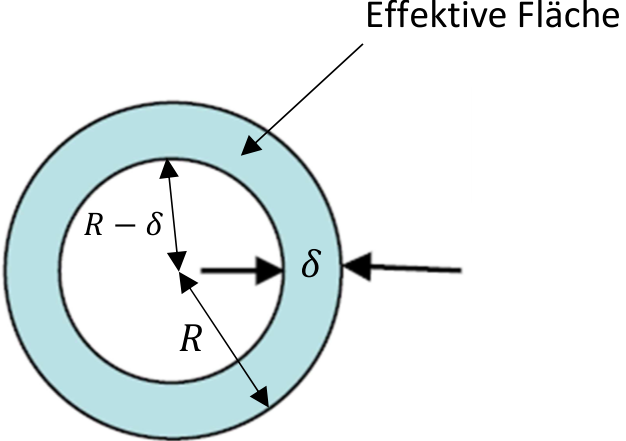
\includegraphics[width=.55\columnwidth]{Figures/Skineffekt.png}\\
%         {\footnotesize$\sigma/\kappa$ : Leitfähigkeit. $[\si{A/Vm}] = [\si{1/\Omega m}]$}
%     \end{minipage}
% }

%\vspace{2cm}

\tikz{
    %Kreise
    \draw[-] (0,0) circle (1);              %äußerer Kreis
    \draw[-] (0,0) circle (0.6);            %innerer Kreis

    %Pfeile
    \draw[latex-latex] (-0.6,0) -- (0,0) node[midway, above]{\tiny{R-$\delta$}};
    \draw[latex-latex] (0,-1) -- (0,0) node at (0,-0.4) [left]{\tiny R};

    \node at (0.8,0)[]{\footnotesize$\delta$};
    \draw[-latex] (0.3,0) -- (0.6,0);
    \draw[latex-] (1,0) -- (1.3,0);

    \draw[latex-] (0.566,0.566) -- (1.2,1.2) node[above, right]{\scriptsize{Effektive Fläche}};

    %Legende
    \node at (-0.8,-1.3)[]{\footnotesize{$\sigma/\kappa$ : Leitfähigkeit [A/Vm] = [1/$\Omega$m]}}




    %--------------------------------------------------------------------
    % %Linien
    % \draw[-] (1,0) -- (1,6);
    % \draw[-] (5,0) -- (5,6);

    % %Pfeile mit Bezeichnungen
    % \draw[->] (3.5,6.5) -- (5,6.5)node[right]{$z$};

    % \draw[->] (1,6) -- (5,5) node[right]{$t_D$} node[midway, above]{$U_{1h}$};
    % %\draw[-] (1,6) -- (3,5.5) node[above]{$U_{1h}$};

    % \draw[->] (5,5) -- (1,4)node[left]{$2t_D$} node[midway, above]{$U_{1r}$};
    % %\draw[-] (5,5) -- (3,4.5) node[above]{$U_{1r}$};

    % \draw[->] (1,4) -- (5,3)node[right]{$3t_D$} node[midway, above]{$U_{2h}$};
    % %\draw[-] (1,4) -- (3,3.5) node[above]{$U_{2h}$};

    % \draw[->] (5,3) -- (1,2)node[left]{$4t_D$} node[midway, above]{$U_{2r}$};
    % %\draw[-] (5,3) -- (3,2.5) node[above]{$U_{2r}$};

    % \draw[->] (1,2) -- (5,1)node[right]{$5t_D$} node[midway, above]{$U_{3h}$};
    % %\draw[-] (1,2) -- (3,1.5) node[above]{$U_{3h}$};


    % \draw[dotted ] (5,1) -- (3,0.5);

    % %Klammern mit Bezeichnungen
    % \draw [black,
    %     decorate,
    %     decoration = {brace,
    %             raise=5pt,
    %             amplitude=5pt}] (1,4.2) --  (1,5.8);
    % \node at(0.5,5)[left]{$U_{1h}$};

    % \draw [black,
    %     decorate,
    %     decoration = {brace,
    %             raise=5pt,
    %             amplitude=5pt}] (5,4.8) --  (5,3.2);
    % \node at (5.5,4)[right]{$U_{1h}(1+r_A)$};

    % \draw [black,
    %     decorate,
    %     decoration = {brace,
    %             raise=5pt,
    %             amplitude=5pt}] (1,2.2) --  (1,3.8);
    % \node at (0.5,3)[left]{$U_{1h}$};
    % \node at (0.5,2.5)[left]{$+(1+r_I)U_{1r}$};

    % \draw [black,
    %     decorate,
    %     decoration = {brace,
    %             raise=5pt,
    %             amplitude=5pt}] (5,2.8) --  (5,1.2);
    % \node at (5.5,2)[right]{$U_{1h}(1+r_A)$};
    % \node at (5.5,1.5)[right]{$+U_{2h}(1+r_A)$};


    % \draw [black,
    %     decorate,
    %     decoration = {brace,
    %             raise=5pt,
    %             amplitude=5pt}] (1,0.2) --  (1,1.8);
    % \node at (0.5,1.5)[left]{$U_{1h}$};
    % \node at (0.5,1)[left]{$+(1+r_I)U_{1r}$};
    % \node at (0.5,0.5)[left]{$+(1+r_I)U_{2r}$};

}

\begin{description}
    \item Äquivalente Leiterschichtdicke (Amp: $A \cdot \frac{1}{e}$):
          \[
              \delta = \frac{1}{\sqrt{\pi\mu\sigma f}} = \sqrt{\frac{2}{\omega\mu\sigma}} \qquad \left[ m \right] \\
          \]

    \item Widerstand/Oberflächenwiderstand:
          \begin{flalign*}
              R_{r\ll\delta}     & = \frac{l}{\sigma \cdot A_{\texttt{eff}}} \\
              R_{r\approx\delta} & =\dfrac{4l}{\sigma \pi d^{2}}             \\
              R_F                & = \dfrac{1}{\sigma \delta}
          \end{flalign*}

    \item \textbf{Feldstärke} verglichen mit der Oberfläche:\\
          \makebox[0pt][l]{
              \begin{minipage}{0.5\columnwidth}
                  \centering
                  \[
                      H\left( x,t\right) = H_{0}\cdot e^{^{-x}/_\delta}\cdot \cos \left( \omega t-\dfrac{x}{\delta}\right)
                  \]
                  \footnotesize analog für $E$-Feld
              \end{minipage}
          }

    \item \textbf{Leistung} verglichen mit der Oberfläche:
          \[
              P\left( x,t\right) = \dfrac{1}{2} \cdot E_{0}\cdot e^{^{-x}/_\delta}\cdot H_{0}\cdot e^{^{-x}/_\delta}
          \]

    \item Amplitude und Phase bezogen auf $\delta$:
          \begin{align*}
              \text{Amplitude: } x   & =\delta \cdot \ln(\text{Dämpfung[ ]}) \\
              \text{Phase: } \varphi & = -\frac{x}{\delta}
          \end{align*}

    \item Effektive Fläche:
          \begin{align*}
              A_{\texttt{eff}} & = A_{\texttt{ges}} - A_{\sigma} = R^2\pi-(R-\sigma)^2\pi \\
                               & = 2\cdot \pi \delta \left( R-\dfrac{\delta }{2}\right)
          \end{align*}
\end{description}

Wenn die Länge nicht gegeben ist oder nach Wieviel \% nimmt der Widerstand bei
einer bestimmten Frequenz, kann dies mit der folgenden Formel berechnet werden:

\begin{description}
    \item Bessel-Funktion:
          \begin{align*}
              \frac{R_{AC}}{R_{DC}} & =
              \begin{dcases}
                  1 + \frac{1}{3}x^4              & \text{für} \qquad x < 1 \\
                  x + \frac{1}{4} + \frac{3}{64x} & \text{für} \qquad x > 1 \\
              \end{dcases} \\
              \frac{X_{AC}}{R_{DC}} & =
              \begin{dcases}
                  x^2\left( 1-\frac{x^4}{6} \right)   & \text{für} \qquad x < 1 \\
                  x- \frac{3}{64x} + \frac{3}{128x^2} & \text{für} \qquad x > 1 \\
              \end{dcases}
          \end{align*}
          \[
              \boxed{x=\frac{r_0}{2\delta}} \qquad r_0 \hat{=} \textnormal{ Außendurchmesser}
          \]
\end{description}

    \section{Wellen}
\begin{itemize}
    \setlength\itemsep{1pt}
    \item Ausbreitungsphänomen von E und H
    \item Ausbreitungsgeschw. kleiner $c_0$
    \item raumzeitlicher Vorgang $cos(\omega t- \beta z)$
    \item Energie- ohne Materietransport
    \item Poyntingvektor $\vec{S}=\vec{E}\times\vec{H}$ Einheit[S]$= \dfrac{W}{m^2}$\\
          {\footnotesize Falls $\vec{E}\perp\vec{H}$ und $\vec{S}\perp\vec{E}$ und $\vec{S}\perp\vec{H}$}
\end{itemize}

\subsubsection*{Wellengleichung}
\makebox[0pt][l]{
    \begin{minipage}{\columnwidth}
        \centering
        \[
            \boxed{\vec{E} = \underbrace{E_0}_{\mathclap{\text{Amplitude}}}
            \cdot \overbrace{e^{-\alpha z}}^{\mathclap{\text{Dämpfung}}}
            \cdot \underbrace{cos(\omega t \overbrace{-}^{\mathclap{\text{positive z-Richtung}}} \beta z)}_\text{Zeit- und Raumabhängigkeit}}
        \]
        {\footnotesize Analog für H-Feld}
    \end{minipage}
}

\subsubsection*{Fortpflanzungskonstante $\gamma$}
\[\boxed{\underline{\gamma}=\alpha+j\beta}\]

$\alpha$ : Dämpfungskonstante [Np/m]

$\beta$ : Phasenkonstante [rad/m]

$v$ : Phasengeschwindigkeit [m/s]

\subsection{Ausbreitung}
\subsubsection{Allgemein}
\begin{align*}
    \lambda                 & = \dfrac{2\pi}{\beta} \qquad E_2 = E_1 e^{-\alpha z}                                                                                        \\
    v_{ph}                  & = \lambda\cdot f                                                                                                                            \\
    \alpha                  & = \omega \cdot \sqrt{\dfrac{\mu \varepsilon}{2}\cdot \left(\sqrt{1+\dfrac{\sigma^2}{\omega^2\cdot\varepsilon^2}}{\color{red}{-}}1\right)}   \\
    \beta                   & = \omega \cdot \sqrt{\dfrac{\mu \varepsilon}{2}\cdot \left(\sqrt{1+\dfrac{\sigma^2}{\omega^2\cdot\varepsilon^2}}{\color{green}{+}}1\right)} \\
    \Aboxed{\underline{Z}_F & = \dfrac{\underline{E}_\text{transversal}}{\underline{H}_\text{transversal}} = \sqrt{\dfrac{j\omega\mu}{\sigma+j\omega\varepsilon}}}        \\
\end{align*}

\subsubsection{Im leeren Raum(Vakuum)}
\begin{align*}
    \alpha                     & = 0                                                    \\
    \beta                      & = \dfrac{\omega}{c_0}                                  \\
    \lambda                    & = \dfrac{c_0}{f}                                       \\
    v                          & = c_0                                                  \\
    \Aboxed{\underline{Z}_{F0} & = \sqrt{\dfrac{\mu_0}{\varepsilon_0}}\approx377\Omega}
\end{align*}

\subsubsection{Im verlustlosen/idealen Dielektrika}
verlustlos: $\sigma =0$, maximale Wirkleistung

$Z_F$ rein reel $\rightarrow$ ebene Welle
\begin{align*}
    \alpha                  & = 0                                                                                              \\
    \beta                   & = \dfrac{\omega}{c_0}\sqrt{\mu_r\varepsilon_r}=\omega\sqrt{\mu\varepsilon}=\dfrac{2\pi}{\lambda} \\
    \lambda                 & = \dfrac{c_0}{f}\dfrac{1}{\sqrt{\mu_r\varepsilon_r}}                                             \\
    v                       & = \dfrac{c_0}{\sqrt{\mu_r\varepsilon_r}}                                                         \\
    \Aboxed{\underline{Z}_F & = \sqrt{\dfrac{\mu}{\varepsilon}}}
\end{align*}

\subsubsection{Im Dielektrika mit geringem Verlust}
geringer Verlust: $0 < \sigma \ll\omega\varepsilon$

\begin{align*}
    \alpha                  & = \dfrac{\sigma}{2}\cdot\sqrt{\dfrac{\mu}{\varepsilon}} = \frac{\sigma}{2}\cdot Z_{F0}               \\
    \beta                   & = \omega\sqrt{\mu\varepsilon}\left(1+\dfrac{1}{8}\cdot\dfrac{\sigma^2}{\omega^2\varepsilon^2}\right) \\
    \lambda                 & = \dfrac{c_0}{f}\cdot\dfrac{1}{\sqrt{\mu_r\varepsilon_r}}                                            \\
    v                       & = \dfrac{c_0}{\sqrt{\mu_r\varepsilon_r}}                                                             \\
    \Aboxed{\underline{Z}_F & = \sqrt{\dfrac{\mu}{\varepsilon}}}
\end{align*}

\subsubsection{Im guten Leiter}
geringer Verlust: $\sigma \gg\omega\varepsilon$
\begin{align*}
    \alpha                  & = \beta = \dfrac{1}{\delta} \sim \sqrt{f}                             \\
    \lambda                 & = 2\pi \sqrt{\dfrac{2}{\omega\mu\sigma}}=2\pi\delta                   \\
    \Aboxed{\underline{Z}_F & = \sqrt{\dfrac{j\omega\mu}{\sigma}} = \dfrac{1+j}{\sigma\cdot\delta}}
\end{align*}

\subsection{Übergang}
\subsubsection{Zwischen Dielektrika mit geringem Verlust}

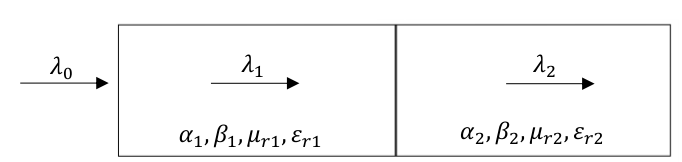
\includegraphics[width=\columnwidth]{Figures/UebergangzweiDielektrika.png}
\begin{align*}
    \quad \qquad \lambda_1 & = \dfrac{\lambda_0}{\sqrt{\mu_{r1}\varepsilon_{r1}}}          & \lambda_2 & = \dfrac{\lambda_0}{\sqrt{\mu_{r2}\varepsilon_{r2}}}                                     \\
    \quad \qquad           &                                                               &           & = \dfrac{\lambda_1\cdot\sqrt{\mu_{r1}\varepsilon_{r1}}}{\sqrt{\mu_{r2}\varepsilon_{r2}}} \\
    \quad \qquad \beta_1   & = \dfrac{2\pi}{\lambda_0}\cdot\sqrt{\mu_{r1}\varepsilon_{r1}} & \beta_2   & = \dfrac{2\pi}{\lambda_0}\cdot\sqrt{\mu_{r2}\varepsilon_{r2}}                            \\
    \quad \qquad Z_{F1}    & = \dfrac{Z_{F0}}{\sqrt{\mu_{r1}\varepsilon_{r1}}}             & Z_{F2}    & = \dfrac{Z_{F0}}{\sqrt{\mu_{r2}\varepsilon_{r2}}}
\end{align*}

\subsection{Energie und Poyntingvektor (Energieflussdichte)}
\begin{align*}
     & \vec{S} = \vec{E}\times\vec{H} \text{ in } [W/m^2]                                   \\
     & S = 1/2 \cdot E \cdot H = 1/2 \cdot \dfrac{E^2}{Z_{F0}} = 1/2 \cdot H^2 \cdot Z_{F0} \\
     & \underline{S}_{\texttt{Mittel}} = 1/2 \cdot Re\{\vec{E}\times\vec{H}^*\}             \\
     & S = \dfrac{P}{A}                                                                     \\
\end{align*}

\subsubsection{Leistung nach Dämpfung}
\begin{align*}
     & P_1 = P_0 \cdot e^{-2\alpha z}                              \\
     & P = \dfrac{\hat{U}^2}{2 Z_L} \text{vom Kabel transportiert}
\end{align*}

\subsection{dÀlembertsche Gleichung (allg.)}
\begin{align*}
    \Delta \vec{E}-\kappa \mu \frac{\partial \vec{E}}{\partial t}-\varepsilon \mu \frac{\partial^{2} \vec{E}}{\partial t^{2}} & = \operatorname{grad} \frac{\rho}{\varepsilon} \\
    \Delta \vec{H}-\kappa \mu \frac{\partial \vec{H}}{\partial t}-\varepsilon \mu \frac{\partial^{2} \vec{H}}{\partial t^{2}} & = 0
\end{align*}

Isolator, ideales Dielektrikum, Nichtleiter $\kappa = 0$
\begin{align*}
    \Delta \vec{E} & =\varepsilon \mu \frac{\partial^{2} \vec{E}}{\partial t^{2}}+\operatorname{grad} \frac{\rho}{\varepsilon} \\
    \Delta \vec{H} & =\varepsilon \mu \frac{\partial^{2} \vec{H}}{\partial t^{2}}
\end{align*}

sehr gute Leiter
\begin{align*}
    \Delta \vec{E} & =\kappa \mu \frac{\partial \vec{E}}{\partial t}+\operatorname{grad} \frac{\rho}{\varepsilon} \\
    \Delta \vec{H} & =\kappa \mu \frac{\partial \vec{H}}{\partial t}
\end{align*}

\subsection{Helmholtz-Gleichungen (Frequenzbereich)}
\begin{align*}
    \Delta \underline{\vec{E}}-\left(\kappa \mu \cdot \mathrm{j} \omega-\varepsilon \mu \cdot \omega^{2}\right) \cdot \underline{\vec{E}} & = \operatorname{grad} \frac{\rho}{\varepsilon} \\
    \Delta \underline{\vec{H}}-\left(\kappa \mu \cdot \mathrm{j} \omega-\varepsilon \mu \cdot \omega^{2}\right) \cdot \underline{\vec{H}} & = 0
\end{align*}

\subsubsection{Zeitbereich}
\begin{align*}
    \Delta \vec{E}-\varepsilon \mu \frac{\partial^{2} \vec{E}}{\partial t^{2}} & =0 \\
    \Delta \vec{H}-\varepsilon \mu \frac{\partial^{2} \vec{H}}{\partial t^{2}} & =0
\end{align*}

\subsubsection{Frequenzbereich (harmonisch)}
\begin{align*}
    \Delta \underline{\vec{E}}+\varepsilon \mu \omega^{2} \cdot \underline{\vec{E}} & =0 \\
    \Delta \underline{\vec{H}}+\varepsilon \mu \omega^{2} \cdot \underline{\vec{H}} & =0
\end{align*}

%%%%%%%%%%%%%%%%%

\subsection{Wellenzahl}
Im Vakuum: $k_{0}=\frac{\omega}{c_{0}}$
\begin{align*}
    k & = \frac{\omega}{v_{p h}} = \frac{2 \pi f}{v_{p h}} = |\vec{k}|                                                              \\
      & = \frac{\omega \cdot n}{c_{0}} = n \cdot k_{0}=\frac{1}{\sqrt{\mu_{r} \cdot \varepsilon_{r}}} \cdot k_{0}=k_{r} \cdot k_{0}
\end{align*}

\subsection{Wellenlänge}
\begin{align*}
    \lambda   & = \dfrac{\lambda_0}{\sqrt{\mu_r \cdot \varepsilon_r}} = \dfrac{2 \pi}{k} = \dfrac{v_{ph}}{f} = [m] \\
              & = \dfrac{\lambda_0}{n} = \dfrac{2 \pi}{n \cdot k_0}                                                \\
    \lambda_0 & = \dfrac{c_0}{f} = \dfrac{2\pi}{k_0}
\end{align*}

\subsection{Phasengeschwindigkeit}
\[
    \dfrac{d z}{d t} = \upsilon_{ph} = c = \dfrac{\omega}{k} = \frac{1}{\sqrt{ \mu_r \mu_0 \varepsilon_r \varepsilon_0}} \qquad \upsilon_{ph,\texttt{Medium} \leq c_0}
\]

\subsubsection{Gruppengeschwindigkeit}
\[
    \upsilon_{g} = \dfrac{d \omega}{d k} = \dfrac{\textnormal{Wegstück der Wellengruppe}}{\textnormal{Laufzeit der Wellengruppe}}
\]

\subsection{Polarisation}
\begin{tabularx}{0.45\textwidth}{>{\hsize=.27\hsize}X|>{\hsize=.5\hsize}X|>{\hsize=.23\hsize}X}
    Lineare      & wenn der Endpunkt des E–Vektors eine Linie beschreibt & $H$ oder $E$ \\
    \hline
    Elliptische  & Endpunkt des E-Vektors eine Ellipse beschreibt        & $E\neq H$    \\
    \hline
    Kreisförmige & der Endpunkt des E-Vektors einen Kreis beschreibt     & $E = H$      \\
\end{tabularx}

\subsubsection{Senkrechte Polarisation}

\begin{tikzpicture}
    \draw[dotted] (-3,0) -- (3,0);
    \draw[-] (0,-4) -- (0,4)                node[below right] {$\varepsilon_{r2}, \mu_{r2}, \sigma_{r2}$}
                                            node[below left] {$\varepsilon_{r1}, \mu_{r1}, \sigma_{r1}$};

    \draw[->] (-3,3) -- (-1.5,1.5)          node[above right] {$S_h$};
    \draw[->] (-3,3) -- (-3.5,2.5)          node[below right] {$H_h$};
    \draw[-] (-3,3) circle (0.15)           node[above] {$E_h$};
    \draw[dotted] (-3,3) -- (0,0);
    \draw[<->] (135:0.5) arc (135:180:0.5); 
    \node[] at (-0.8,0.2) {$\alpha$};

    \draw[->] (-1.5,-1.5) -- (-2,-2)        node[above left] {$S_r$};
    \draw[->] (-1.5,-1.5) -- (-1.8,-1.2)    node[above] {$H_r$};
    \draw[-] (-1.5,-1.5) circle (0.15)      node[right] {$E_r$};
    \draw[dotted] (-3,-3) -- (0,0);
    \draw[<->] (180:0.5) arc (180:225:0.5);
    \node[] at (-0.8,-0.2) {$\alpha$};

    \draw[->] (2,-0.6666) -- (3,-1)         node[above right] {$S_g$};
    \draw[->] (2,-0.6666) -- (1.3333,-2.8)  node[below right] {$H_g$};
    \draw[-] (2,-0.6666) circle (0.15)      node[above] {$E_g$};
    \draw[dotted] (0,0) -- (3,-1);
    \draw[<->] (0:1) arc (0:-20:1);     
    \node[] at (1.3,-0.2) {$\beta$};

\end{tikzpicture}

\begin{itemize}
    \item mag./elek. Reflexionsfaktor $[1]$
    \item mag. Transmissionsfaktor $[1]$
    \item elek. Transmissionsfaktor $[1]$
\end{itemize}

\begin{align*}
    r_{m s} & = \frac{Z_{F 2} \cdot \cos \alpha-Z_{F 1} \cdot \cos \beta}{Z_{F 2} \cdot \cos \alpha+Z_{F 1} \cdot \cos \beta} = r_{e s} = r_{s} \\
    t_{m s} & = \frac{2 \cdot Z_{F 1} \cdot \cos \alpha}{Z_{F 2} \cdot \cos \alpha+Z_{F 1} \cdot \cos \beta}                                    \\
    t_{e s} & = \frac{2 \cdot Z_{F 2} \cdot \cos \alpha}{Z_{F 2} \cdot \cos \alpha+Z_{F 1} \cdot \cos \beta}                                    \\
    t_{e s} & -r_{e s}= 1 \qquad t_{m s} = (1 - r_{m s}) \cdot \dfrac{\cos \alpha}{\cos \beta}                                                  \\
    E_{g}   & = t_{e s} \cdot E_{h} \qquad E_{r} = r_{s} \cdot E_{h}                                                                            \\
    H_{g}   & = t_{m s} \cdot H_{h} \qquad H_{r} = r_{s} \cdot H_{h}
\end{align*}

\subsubsection{Parallel Polarisation}
\begin{tikzpicture}
    \draw[dotted] (-3,0) -- (3,0);
    \draw[-] (0,-4) -- (0,4)                node[below right] {$\varepsilon_{r2}, \mu_{r2}, \sigma_{r2}$}
                                            node[below left] {$\varepsilon_{r1}, \mu_{r1}, \sigma_{r1}$};

    \draw[->] (-3,3) -- (-1.5,1.5)          node[above right] {$S_h$};
    \draw[->] (-3,3) -- (-3.5,2.5)          node[below right] {$E_h$};
    \draw[-] (-3,3) circle (0.15)           node[above] {$H_h$};
    \draw[dotted] (-3,3) -- (0,0);
    \draw[<->] (135:0.5) arc (135:180:0.5); 
    \node[] at (-0.8,0.2) {$\theta_h$};

    \draw[->] (-1.5,-1.5) -- (-2,-2)        node[above left] {$S_r$};
    \draw[->] (-1.5,-1.5) -- (-1.8,-1.2)    node[above] {$E_r$};
    \draw[-] (-1.5,-1.5) circle (0.15)      node[right] {$H_r$};
    \draw[dotted] (-3,-3) -- (0,0);
    \draw[<->] (180:0.5) arc (180:225:0.5);
    \node[] at (-0.8,-0.2) {$\theta_r$};

    \draw[->] (2,-0.6666) -- (3,-1)         node[above right] {$S_t$};
    \draw[->] (2,-0.6666) -- (1.3333,-2.8)  node[below right] {$E_t$};
    \draw[-] (2,-0.6666) circle (0.15)      node[above] {$H_t$};
    \draw[dotted] (0,0) -- (3,-1);
    \draw[<->] (0:1) arc (0:-20:1);     
    \node[] at (1.3,-0.2) {$\theta_t$};

\end{tikzpicture}

\begin{itemize}
    \item mag./elek. Reflexionsfaktor $[1]$
    \item mag. Transmissionsfaktor $[1]$
    \item elek. Transmissionsfaktor $[1]$
\end{itemize}

\begin{align*}
    r_{m p} & = \frac{Z_{F 1} \cos \vartheta_{1}-Z_{F 2} \cos \vartheta_{2}}{Z_{F 1} \cos \vartheta_{1}+Z_{F 2} \cos \vartheta_{2}} = r_{e p} = \frac{E_{r 0}}{E_{h 0}} =r_{p} \\
    t_{m p} & = \frac{2 Z_{F 1} \cos \vartheta_{1}}{Z_{F 1} \cos \vartheta_{1}+Z_{F 2} \cos \vartheta_{2}}                                                                     \\
    t_{e p} & = \frac{2 Z_{F 2} \cos \vartheta_{1}}{Z_{F 1} \cos \vartheta_{1}+Z_{F 2} \cos \vartheta_{2}} = \frac{Z_{F 2}}{Z_{F 1}} t_{m p}
\end{align*}

    \section{Leitungen}
\subsection{Leitungsparameter}

{\small\[
        \sigma = \text{Leitwert des Dielektr.} \qquad \sigma_c = \text{Leitwert des Leiters}
    \]}

\subsubsection{Doppelleitung:}
{\small\[
        a = \text{Leiter Radius} \qquad d = \text{Abstand zw. den Leitern} \\
    \]}

\begin{tikzpicture}
    \tikzset{cross/.style={cross out, draw=black, minimum size=2*(#1-\pgflinewidth), inner sep=0pt, outer sep=0pt},
        %     %default radius will be 1pt. 
        cross/.default={3.5pt}}

        %linker Außenleiter
        \draw[-](-0.53,0.53)--(0.97,2.03);

        
        \draw[-](48:0.75) arc (48:312:0.75);

        %linker Innenleiter
        \draw[dashed](-0.106,0.106)--(0.41,0.622);
        \draw[dashed](0.106,-0.106)--(0.922,0.71);

        \draw[-](0,0) circle (0.15);
        \draw(0,0) node [cross] {};


        
        %%%%%%%%%%%%%%%%%%%%%%%%%%%%%%%%%%%%%%%%%%%%%%%%%%%%%%%%%%%
        %%%%%%%%%%%%%%%%%%%%%%%%%%%%%%%%%%%%%%%%%%%%%%%%%%%%%%%%%%%

        %Rechter Außenleiter
        \draw[-](0.48,0.58)--(1.97,2.03);
        \draw[-](1.53,-0.53)--(2.63,0.57);

        %Rechter Innenleiter
        \draw[dashed](0.894,0.106)--(1.41,0.622);
        \draw[dashed](1.106,-0.106)--(1.622,0.41);

        \draw[-](1,0) circle (0.15);
        \draw[-,fill=black!100] (1,0) circle (0.05);

        \draw([shift={(228:0.75)}]1,0) arc (-132:132:0.75);

\end{tikzpicture}

{\renewcommand*{\arraystretch}{0.2}
    \begin{tabularx}{0.5\columnwidth}{|X|}
        \hline
        \[R  = \frac{1}{\pi a\delta\sigma_c}\]              \\
        \hline
        \[L = \frac{\mu}{\pi} \cosh^{-1}\frac{d}{2a}\]      \\
        \hline
        \[G = \frac{\pi\sigma}{\cosh^{-1}(^d/_{2a})}\]      \\
        \hline
        \[C = \frac{\pi\varepsilon}{\cosh^{-1}(^d/_{2a})}\] \\
        \hline
    \end{tabularx}}

\subsubsection{Koaxial Leitung}
{\small\[
        a = \text{innen Radius} \qquad b = \text{außen Radius} \\
    \]}

\begin{align*}
    \vec{H}(r, z) & = \frac{I}{2\pi r}\cdot e^{-j\beta z}\cdot\vec{e}_\varphi                    \\
    \vec{E}(r, z) & = \frac{I}{2\pi r}\cdot Z_F\cdot e^{-j\beta z} \cdot\vec{e}_r                \\
                  & = \frac{\hat{U}}{r \cdot\ln{(^{2b}/_{2a})}}\cdot e^{-j\beta z}\cdot\vec{e}_r
\end{align*}

\begin{tikzpicture}
    \tikzset{cross/.style={cross out, draw=black, minimum size=2*(#1-\pgflinewidth), inner sep=0pt, outer sep=0pt},
        %     %default radius will be 1pt. 
        cross/.default={3.5pt}}

        %Außenleiter
        \draw[-](-0.53,0.53)--(0.97,2.03);
        \draw[-](0.53,-0.53)--(1.63,0.57);

        \draw[-](0,0) circle (0.75);

        %Innenleiter
        \draw[-](-0.106,0.106)--(0.41,0.622);
        \draw[-](0.106,-0.106)--(0.622,0.41);

        \draw[-](0,0) circle (0.15);
        \draw(0,0) node [cross] {};

\end{tikzpicture}
{\renewcommand*{\arraystretch}{0.2}
    \begin{tabularx}{0.5\columnwidth}{|X|}
        \hline
        \[R=\frac{1}{2\pi\delta\sigma_c}\left[\frac{1}{a}+\frac{1}{b}\right]\] \\
        \hline
        \[L=\frac{\mu}{2\pi}\ln\frac{b}{a}\]                                   \\
        \hline
        \[G=\frac{2\pi\sigma}{\ln(^b/_a)}\]                                    \\
        \hline
        \[C=\frac{2\pi\varepsilon}{\ln(^b/_a)}\]                               \\
        \hline
    \end{tabularx}}

\subsubsection{Parallele Platten}
{\small\[
        w  = \text{Platten Breite} \qquad d  = \text{Abstand zw. Platten}
    \]}

\begin{tikzpicture}
    \tikzset{cross/.style={cross out, draw=black, minimum size=2*(#1-\pgflinewidth), inner sep=0pt, outer sep=0pt},
        %     %default radius will be 1pt. 
        cross/.default={3.5pt}}

        %Untereplatte
        \draw[-](0,0)--(0,0.35);
        \draw[-](2,0)--(2,0.35);

        \draw[-](0,0)--(2,0);
        \draw[-](0,0.35)--(2,0.35);

        \draw[-](0,0.35)--(0.3,0.65);
        \draw[-](2,0)--(2.75,0.75);
        \draw[-](2,0.35)--(2.75,1.15);

        \draw[-](1,0.175) circle (0.15);
        \draw[-,fill=black!100] (1,0.175) circle (0.05);

        %Obere Platte
        \draw[-](0,0.65)--(0,1);
        \draw[-](2,0.65)--(2,1);

        \draw[-](0,0.65)--(2,0.65);
        \draw[-](0,1)--(2,1);

        \draw[-](0,1)--(0.75,1.75);
        \draw[-](2,1)--(2.75,1.75);
        \draw[-](2,0.65)--(2.75,1.4);

        \draw[-](1,0.825) circle (0.15);
        \draw(1,0.825) node [cross] {};
   
\end{tikzpicture}

{\renewcommand*{\arraystretch}{0.2}
    \begin{tabularx}{0.5\columnwidth}{|X|}
        \hline
        \[R=\frac{2}{w\delta\sigma}\] \\
        \hline
        \[L=\frac{\mu d}{w}\]         \\
        \hline
        \[G=\frac{\sigma w}{d}\]      \\
        \hline
        \[C=\frac{w\varepsilon}{d}\]  \\
        \hline
    \end{tabularx}
}

\textbf{\color{red}{Leitungen gehen HIN und ZURÜCK!!!}\\
    \color{red}{Länge verdoppeln!!!}
}

\vspace{1ex}
Für beliebige Leitergeometrie gelten folgende Zusammenhänge:
\[
    LC = \mu\varepsilon \quad \text{und} \quad \frac{G}{C} = \frac{\sigma}{\varepsilon}
\]

\subsection{Allgemeine Lösung Leitungsgleichung}
\begin{align*}
    \underline{U}(z)   & = U_h e^{\underline{\gamma} z} + U_r e^{-\underline{\gamma} z} = U_h e^{\underline{\gamma} d} + U_r e^{-\underline{\gamma} d}                       \\
    \underline{I}(z)   & = I_h e^{\underline{\gamma} z} + I_r e^{-\underline{\gamma} z} = \frac{U_h}{Z_L}e^{\underline{\gamma} d} - \frac{U_r}{Z_L}e^{-\underline{\gamma} d} \\
    \underline{Z}_L    & = \frac{U_h}{I_h} = \sqrt{ \frac{R + j \omega L}{G + j \omega C}}                                                                                   \\
    \underline{\gamma} & = j \omega \sqrt{LC} \cdot \sqrt{ \frac{RG}{j^2 \omega^2 LC} + \frac{G}{j \omega C} + \frac{R}{j \omega L} + 1}                                     \\
    \lambda            & = \frac{2 \pi}{\beta}                                                                                                                               \\
    v_{Ph}             & = \frac{\omega}{\beta}                                                                                                                              \\
    l_\texttt{elektr.} & = \beta \cdot l                                                                                                                                     \\
    \alpha             & = \omega \cdot \sqrt{\dfrac{\mu \varepsilon}{2}\cdot \left(\sqrt{1+\dfrac{\sigma^2}{\omega^2\cdot\varepsilon^2}}{\color{red}{-}}1\right)}           \\
    \beta              & = \omega \cdot \sqrt{\dfrac{\mu \varepsilon}{2}\cdot \left(\sqrt{1+\dfrac{\sigma^2}{\omega^2\cdot\varepsilon^2}}{\color{green}{+}}1\right)}
\end{align*}

\subsubsection{Verlustlose Übertragungsleitung}
\begin{align*}
    \underline{\gamma} & = j\omega\sqrt{LC}= j\beta                                                                                           \\
    Z_L                & =\frac{U_h}{U_r}       = \sqrt{\frac{L}{C}}                                                                          \\
    v                  & = \frac{\omega}{\beta} = \frac{1}{\sqrt{LC}}= \frac{1}{\sqrt{\mu\varepsilon}}= \frac{c_0}{\sqrt{\mu_r\varepsilon_r}} \\
    \lambda            & = \frac{2\pi}{\beta}=\frac{1}{f\sqrt{LC}}= \frac{v}{f}= \frac{c_0}{f\sqrt{\mu_r\varepsilon_r}}
\end{align*}

\subsubsection{vernachlässigbarer Widerstandsbelag}
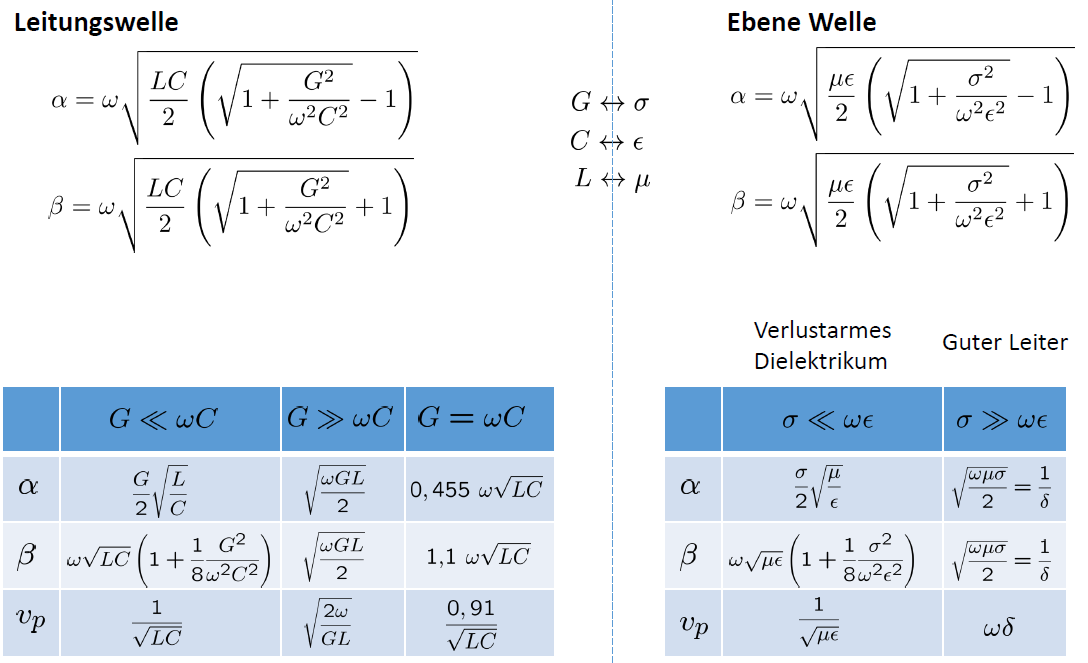
\includegraphics[width=\columnwidth]{Figures/vernachlaessigbarerWiderstandsbelag.png}


\subsubsection{vernachlässigbarer Leitwertbelag}
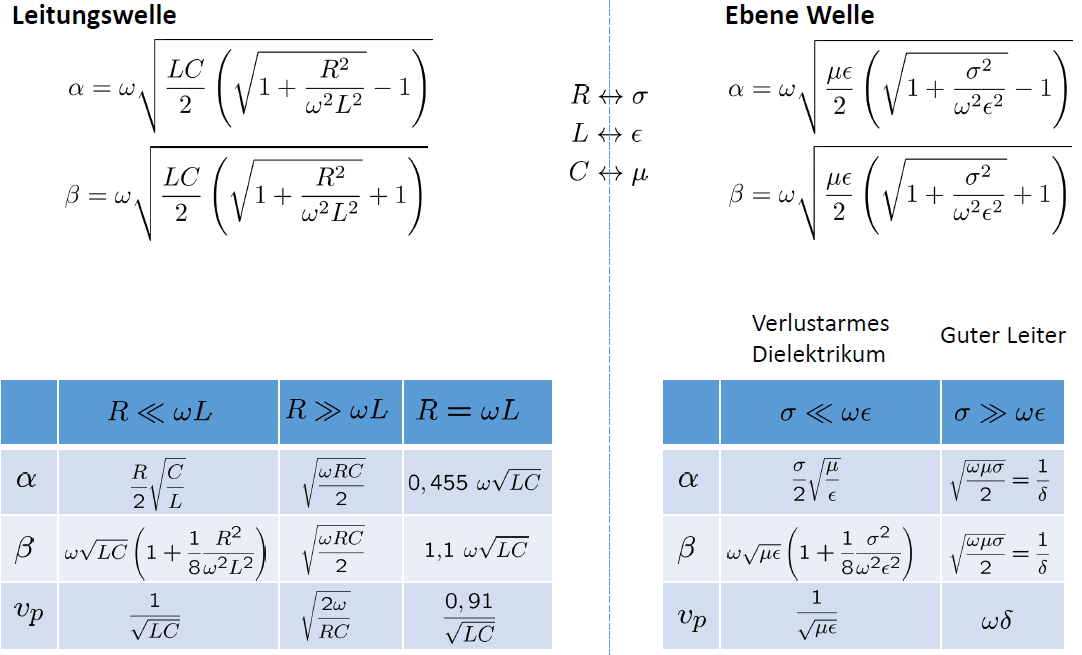
\includegraphics[width=\columnwidth]{Figures/vernachlaessigbarerLeiterwertbelag.png}

\subsection{Übertragungsleitung mit Last}

\def\Hoehe{2};
\def\Breite{8}
\resizebox{0.4\textwidth}{!}{
    %\centering
    \begin{tikzpicture}
        \begin{circuitikz}%[american voltages]
            \draw(0,0)
            to[V,v=$u_G(t)$](0,2)                           %Spannungsquelle
            to[R=$Z_g$](2,2)                               %Quelleninnenwiderstand
            to[short](8,2)
            to[R= $Z_A$](8,0)                               %Lastwiderstand
            to[short](0,0);             
            \draw[-] (2,2) circle (0.1);                    %TOR 1 oben
            \draw[-] (6,2) circle (0.1);                    %TOR 2 oben
            \draw[-] (2,0) circle (0.1);                    %TOR 1 unten
            \draw[-] (6,0) circle (0.1);                    %TOR 2 unten
            \draw[dotted](2,0)--(2,-0.5) node[left]{$l=0$};
            \draw[dotted](2,-0.5)--(2,-1) node[left]{$z=d$};
            \draw[dotted](2,-1)--(2,-1.5);
            \draw[->](2,-0.5) -- (6,-0.5);
            \node at (5,-0,5)[above]{positiv l};

            \draw[dotted](6,0)--(6,-0.5) node[right]{$l=d$};          
            \draw[dotted](6,-0.5)--(6,-1) node[right]{$z=0$};
            \draw[dotted](6,-1)--(6,-1.5);
            \draw[->](6,-1.5) -- (2,-1.5);
            \node at (5,-1,5)[above]{positiv z};

            \draw[->](2,1.25) -- (5,1.25);
            \node at (4,1.25)[above]{forward propagating wave};
            \draw[->](6,0.5) -- (3,0.5);
            \node at (5,0.5)[above]{backward propagating wave};
        \end{circuitikz}
    \end{tikzpicture}
}

\begin{align*}
    U(z) & = U_h\cdot  e^{\underline{\gamma} z} + U_r\cdot  e^{-\underline{\gamma} z} = U_h\cdot  e^{\underline{\gamma} d} + U_r\cdot  e^{-\underline{\gamma} d}           \\
    I(z) & = I_h\cdot  e^{\underline{\gamma} z} + I_r\cdot  e^{-\underline{\gamma} z} = \frac{U_h}{Z_L}e^{\underline{\gamma} d} - \frac{U_r}{Z_L}e^{-\underline{\gamma} d}
\end{align*}

\subsubsection{Vorgehen Eingangswiderstand}
Wenn mit Smithdiagramm gearbeitet wird liefert dieses Schritte \ref{Ref L_anfang} und \ref{Bestimmen Z_E}
\begin{enumerate}
    \item Lastimpedanz
          \[ \underline{Z}_A = \dfrac{1}{\frac{1}{R_A} + j \omega C_A} \]
    \item Reflexion am Leitungsende
          \[ \underline{r}_A = \underline{r}(z=0) = \dfrac{Z_A - \underline{Z}_L}{Z_A + \underline{Z}_L} \]
    \item Reflexion am Leitungsanfang \label{Ref L_anfang}
          \[ \underline{r}_E = \underline{r}(z=d) =  \underline{r}_A \cdot e^{-j 2 \beta d}\]
    \item Bestimmung der Impedanz \label{Bestimmen Z_E}
          \[ \underline{Z}_E = \underline{Z}_L \cdot \dfrac{1 + \underline{r}_E}{1 - \underline{r}_E}\]
    \item Eingangswiderstand
          \[ \underline{Z}_E = \dfrac{1}{\frac{1}{\underline{Z}_E} + j \omega C_E}\]
\end{enumerate}


\subsubsection{Reflexionsfaktor entlang einer Leitung}
\begin{align*}
    r_E    & = r_A  ^{-2\underline{\gamma} l} = r_A  e^{-2\alpha l} e^{-j2\beta l}                                                     \\
    \alpha & = -\frac{\ln(r_A)}{2l} [\si{Np/m}]                                    & \beta & = \dfrac{\phi_2 -\phi_1}{2l} [\si{rad/m}]
\end{align*}

\subsubsection{Stehwellenverhältnis}
\begin{align*}
    \mathrm{SWR} = \frac{U_\text{max}}{U_\text{min}} =
    \frac{I_\text{max}}{I_\text{min}} = \frac{1+|r(z)|}{1-|r(z)|} =
    \frac{|U_H|+|U_R|}{|U_H|-|U_R|}
\end{align*}

\subsubsection{Position von Extrema}
\begin{gather*}
    \boxed{r_A = |r_A|\cdot e^{-j\theta_r}}\rightarrow\theta_r\text{ in rad}\\
    f_\texttt{min}\rightarrow \text{Minimum(Knoten) der Spannungen}\\
    f_\texttt{max}\rightarrow \text{Maximum(Bäuche) der Spannungen}
\end{gather*}
\begin{align*}
    \lambda_\texttt{min/max} & = \frac{c_0}{f_\texttt{min/max}\sqrt{\mu_{r1}\varepsilon_{r1}}}                                                                                                 \\
    z_\texttt{min}           & =\frac{-n\cdot\lambda_\texttt{min}}{2}                                        \qquad\rightarrow n = -\frac{2z}{\lambda_\texttt{min}}                            \\
    z_\texttt{max}           & =\frac{-(2n+1)\lambda_\texttt{max}}{4}                                        \qquad\rightarrow n = -\frac{4z+\lambda_\texttt{max}}{2\cdot\lambda_\texttt{max}} \\
    z                        & = \frac{\lambda_\texttt{min}\cdot\lambda_\texttt{max}}{4(\lambda_\texttt{min}-\lambda_\texttt{max})}
\end{align*}

\vspace{20pt}
\textbf{Spezialfälle auf der nächsten Seiten}
\pagebreak

\subsubsection{Spezialfall: Angepasste Leitung}
\begin{align*}
    Z_A          & = Z_L = Z(z)                              \\
    r_A          & = 0\qquad\rightarrow\text{reflexionsfrei} \\
    \mathrm{SWR} & = 1                                       \\
    U(z)         & = U_h\cdot e ^{j\beta z}                  \\
    I(z)         & = I_h \cdot e^{j\beta z}                  \\
                 & = \frac{U_h}{Z_L}\cdot e^{j\beta z}
\end{align*}

\subsubsection{Spezialfall: Kurzgeschlossene Leitung}
\begin{align*}
    Z_A          & = 0                                                                        \\
    Z(z)         & = j Z_L\cdot\tan(\beta z)        \qquad\rightarrow\text{rein imaginär}     \\
    r_A          & = -1                                                                       \\
    \mathrm{SWR} & = \infty                                                                   \\
    U(z)         & = U_h\cdot 2j\sin(\beta z)    \qquad\rightarrow U(z=0)=0                   \\
    I(z)         & = U_h\cdot 2\cos(\beta z)    \qquad\rightarrow I(z=0)=I_A=\frac{2U_h}{Z_L}
\end{align*}

\subsubsection{Spezialfall: Leerlaufende Leitung}
\begin{align*}
    Z_A          & = \infty                                                                         \\
    Z(z)         & = -jZ_L\cdot \cot(\beta z) \qquad\rightarrow\text{rein imaginär}                 \\
    r_A          & = 1                                                                              \\
    \mathrm{SWR} & = \infty                                                                         \\
    U(z)         & = U_h\cdot 2\cos(\beta z) \qquad\rightarrow U(z=0)=0                             \\
    I(z)         & = U_h\cdot 2j\sin(\beta z) \qquad\rightarrow I(z=0)=I_A = \frac{2\cdot U_h}{Z_L}
\end{align*}

\subsubsection{Spezialfall: Ohm'sch abgeschlossene Leitung}
\[
    r_A = \texttt{reell}
\]

\begin{align*}
    \underline{R_A > Z_L} & \rightarrow\theta_r = 0 \rightarrow r_A \texttt{ ist negativ} \\
                          & \rightarrow z_\texttt{max}=\frac{\lambda}{2}\cdot n
\end{align*}

\begin{align*}
    \underline{R_A < Z_L} & \rightarrow\theta_r = \pi                           \\
                          & \rightarrow z_\texttt{min}=\frac{\lambda}{2}\cdot n
\end{align*}

\columnbreak
\subsection{Mehrfachreflexionen bei fehlender Anpassung}
\begin{center}
    \begin{tikzpicture}
        %Linien
        \draw[-Latex] (1,1) -- (1,0) node [below] {$t$};
        \draw[-,line width=1pt] (1,1) -- (1,6);
        \draw[-,line width=1pt] (5,0) -- (5,6);

        %Pfeile mit Bezeichnungen
        \draw[-Latex] (3.5,6.5) -- (5,6.5)node[right]{$z$};

        \draw[-Latex] (1,6) -- (5,5) node[right]{$t_D$} node[midway, above]{$U_{1h}$};
        %\draw[-] (1,6) -- (3,5.5) node[above]{$U_{1h}$};

        \draw[-Latex] (5,5) -- (1,4)node[left]{$2t_D$} node[midway, above]{$U_{1r}$};
        %\draw[-] (5,5) -- (3,4.5) node[above]{$U_{1r}$};

        \draw[-Latex] (1,4) -- (5,3)node[right]{$3t_D$} node[midway, above]{$U_{2h}$};
        %\draw[-] (1,4) -- (3,3.5) node[above]{$U_{2h}$};

        \draw[-Latex] (5,3) -- (1,2)node[left]{$4t_D$} node[midway, above]{$U_{2r}$};
        %\draw[-] (5,3) -- (3,2.5) node[above]{$U_{2r}$};

        \draw[-Latex] (1,2) -- (5,1)node[right]{$5t_D$} node[midway, above]{$U_{3h}$};
        %\draw[-] (1,2) -- (3,1.5) node[above]{$U_{3h}$};


        \draw[dotted ] (5,1) -- (3,0.5);

        %Klammern mit Bezeichnungen
        \draw [black,
            decorate,
            decoration = {brace,
                    raise=5pt,
                    amplitude=5pt}] (1,4.2) --  (1,5.8);
        \node at(0.5,5)[left]{$U_{1h}$};

        \draw [black,
            decorate,
            decoration = {brace,
                    raise=5pt,
                    amplitude=5pt}] (5,4.8) --  (5,3.2);
        \node at (5.5,4)[right]{$U_{1h}(1+r_A)$};

        \draw [black,
            decorate,
            decoration = {brace,
                    raise=5pt,
                    amplitude=5pt}] (1,2.2) --  (1,3.8);
        \node at (0.5,3)[left]{$U_{1h}$};
        \node at (0.5,2.5)[left]{$+(1+r_I)U_{1r}$};

        \draw [black,
            decorate,
            decoration = {brace,
                    raise=5pt,
                    amplitude=5pt}] (5,2.8) --  (5,1.2);
        \node at (5.5,2)[right]{$U_{1h}(1+r_A)$};
        \node at (5.5,1.5)[right]{$+U_{2h}(1+r_A)$};


        \draw [black,
            decorate,
            decoration = {brace,
                    raise=5pt,
                    amplitude=5pt}] (1,0.2) --  (1,1.8);
        \node at (0.5,1.5)[left]{$U_{1h}$};
        \node at (0.5,1)[left]{$+(1+r_I)U_{1r}$};
        \node at (0.5,0.5)[left]{$+(1+r_I)U_{2r}$};
    \end{tikzpicture}
\end{center}

\begin{align*}
    %u_{1h} & = u_G\cdot\frac{ Z_L}{R_I + Z_L}            \\
    u_{1r} & = r_A\cdot u_{1h}                                \\
    u_{2h} & = r_I\cdot u_{1r} = r_I\cdot r_A\cdot u_{1h}     \\
    u_{2r} & = r_A\cdot u_{2h} = r_I\cdot r_A^2\cdot u_{1h}   \\
    u_{3h} & = r_I\cdot u_{2r} = r_I^2\cdot r_A^2\cdot u_{1h}
\end{align*}
\resizebox{0.4\textwidth}{!}{
    %\centering
    \begin{tikzpicture}
        \begin{circuitikz}%[american voltages]
            \draw(0,0)
            to[V,v=$u_G(t)$](0,2)   %Spannungsquelle
            to[R=$R_I \neq Z_L$](2,2) %Quelleninnenwiderstand
            to[short](8,2)
            to[R= $R_A\neq Z_L$](8,0)
            to[short](0,0)
            (4,2) to [open, v=$u(z\mathpunct{,}t)$] (4,0) %Spannungspfeil u(z,t)
            (2,2) to [open, v=$u_E(t)$] (2,0) %Spannungspfeil u_E(t)
            (6,2) to [open, v=$u_A(t)$] (6,0); %Spannungspfeil u_A(t)
            \draw[-] (2,2) circle (0.1);
            \draw[-] (6,2) circle (0.1);
            \draw[-] (2,0) circle (0.1);
            \draw[-] (6,0) circle (0.1);
        \end{circuitikz}
    \end{tikzpicture}
}
\begin{align*}
     & \text{Reflexionsfaktor Leitungsanfang: } & \underline{r}_I & = \frac{R_I - Z_L}{R_I + Z_L}                 \\
     & \text{Reflexionsfaktor Leitungsende: }   & \underline{r}_A & = \frac{R_A - Z_L}{R_A + Z_L}                 \\
     & \text{Signallaufzeit: }                  & t_d             & = \frac{l}{c_0}\cdot\sqrt{\mu_r\varepsilon_r} \\
     & \text{Hinlaufende Welle}                 & u_{1h}          & = \hat{u}_G \cdot\frac{Z_L}{Z_L+R_I}
\end{align*}


\end{multicols*}

\end{document}
